\chapter{Types and Interfaces}
These type definitions are the foundation of the library.
They are stored inside \mintinline{ts}{enums.ts}.
The \mintinline{ts}{base_id} type is used throughout in the library.
It signifies that the identification variable for a vertex can be either
a string of characters or a number.

\begin{minted}[bgcolor=bg]{typescript}
export type base_id = string | number;
\end{minted}

An ID of \mintinline{ts}{"vertex_a"} is as valid as an ID of 42, for instance.
The \mintinline{ts}{args} interfaces are used by function inputs.
For example, when creating an edge,
the library will be expecting an object with the format of \mintinline{ts}{EdgeArgs}.

The question-mark indicates a property is optional.
Weights are optional parameters, and (as previously mentioned) set to one by default.

\begin{minted}[bgcolor=bg]{typescript}
export interface VertexArgs {
  id: base_id;
  weight?: number;
}

export interface EdgeArgs {
  from: base_id;
  to: base_id;
  id?: base_id;
  weight?: number;
  do_force?: boolean;
}

export interface NetworkArgs {
  is_directed?: boolean;
  edge_limit?: number;
  vertex_limit?: number;
}
\end{minted}

It is possible to create a network without any parameters.
The following is an example of code that creates a network \mintinline{ts}{net},
then adds the vertices `1' and `b' and an edge between them.
It is represented visually in Figure \ref{fig:net_1b}.

\begin{minted}[bgcolor=bg]{typescript}
const net = new Network()

net.addVertex({ id: 1 })
net.addVertex({ id: 'b' })

net.addEdge(1, 'b')
\end{minted}

\begin{figure}[H]
  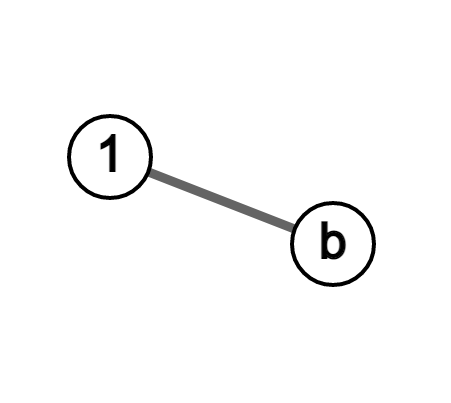
\includegraphics[width=\linewidth]{img/ex_net_1b.png}
  \caption{`net' with an edge between `1' and `b'.}
  \label{fig:net_1b}
\end{figure}

Networks are by default undirected.
A directed network has to be explicitly declared:

\begin{minted}[bgcolor=bg]{typescript}
const is_directed = true
const directed_net = new Network({ is_directed })
net.addEdge(1, 'b')
\end{minted}

\begin{figure}[H]
  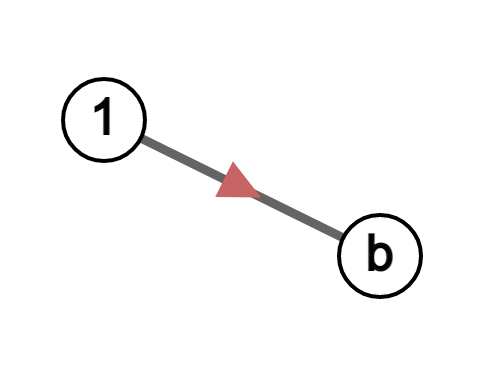
\includegraphics[width=\linewidth]{img/ex_net_1b_dir.png}
  \caption{Network now directed from `1' to `b'}
  \label{fig:net_1b_dir}
\end{figure}

\mintinline{ts}{ParsedCSV} and \mintinline{ts}{ERROR} are types used internally
by the library to load CSV files and manage error messages, respectively.

\begin{minted}[bgcolor=bg]{typescript}
export type ParsedCSV = string[][];

export const ERROR = {...};
\end{minted}

\section{Vertex and Edge Classes}
The vertex class receives an object with the interface of \mintinline{ts}{VertexArgs}.
The weight is optional and, if not provided as a parameter, set to one.

\begin{minted}[bgcolor=bg]{typescript}
import { base_id, VertexArgs } from "./enums.ts";

export class Vertex {
  readonly id: base_id;
  weight: number;

  constructor(args: VertexArgs) {
    this.id = args.id;
    this.weight = args.weight ?? 1;
  }
}
\end{minted}

The \mintinline{ts}{??} operator is a `Nullish coalescing operator' introduced in ES2021.
If \mintinline{ts}{args.weight} is undefined, the instruction on the right is chosen.
This operator is used instead of the ternary \mintinline{ts}{a ? b : c} operator
because, if \mintinline{ts}{args.weight = 0}, it would still select \mintinline{ts}{args.weight},
whereas the ternary operator would consider '0' a Falsy value.

A Falsy value is something with the same Boolean value as false.
For example, '0', although a number, is still considered Falsy in TypeScript.
In other languages, such as Ruby, '0' actually has a Truthy value,
meaning that if you feed it into a logical operation, it evaluates to true.

The edge class has \mintinline{ts}{from} and \mintinline{ts}{to} properties that hold
the ID of a vertex in a network, and a weight that behaves in the same way as the vertex class.
The IDs of the vertices in an edge are private, meaning they cannot be read or overwritten.
When an edge is added to a network, only its weight can be altered from outside the class.

Changing the verticesof an edge would fundamentally change what that edge is and is thus not allowed.
The vertices can be accessed and read through the \mintinline{ts}{vertices} getter,
which returns the edge's \mintinline{ts}{from} and \mintinline{ts}{to} properties:

\begin{minted}[bgcolor=bg]{typescript}
import { base_id, EdgeArgs } from "./enums.ts";

export class Edge {
  private to: base_id;
  private from: base_id;
  weight: number;

  constructor(args: EdgeArgs) {
    this.from = args.from;
    this.to = args.to;
    this.weight = args.weight ?? 1;
  }

  /**
   * Returns an object with the two vertices in the edge.
   * @returns {{ from:base_id, to:base_id }}
   */
  get vertices(): { from: base_id; to: base_id } {
    return { from: this.from, to: this.to };
  }
}
\end{minted}

\section{Network Constructor}

The network class has 4 \mintinline{ts}{readonly} properties.
The edges and vertices are stored in Maps that use \mintinline{ts}{base_id},
as their keys and the values store the actual vertex or edge instance.
The two other \mintinline{ts}{readonly} are Booleans that store fundamental graph properties:
the directionality and complexity of the network.

The \mintinline{ts}{private} properties have to do with hidden functionality
and performance limitations.

There are limits to the number of edges and vertices a network can have,
and they can only be set in the creation of a network.
Most of the time when it is necessary to work with a graph data structure,
the scale of such graphs is already known.
Therefore, to assist with error handling limits to the number of edges and vertices are set.
This helps because it prevents users from getting into infinite loops that try to add
too many edges or vertices.

\begin{minted}[bgcolor=bg]{typescript}
class Network {
  readonly edges: Map<base_id, Edge>;
  readonly vertices: Map<base_id, Vertex>;

  readonly is_directed: boolean;
  readonly is_multigraph: boolean;

  private edge_limit: number;
  private vertex_limit: number;
  private free_eid: number;
  private free_vid: number;

  constructor(args: NetworkArgs = {}) {
    this.edges = new Map();
    this.vertices = new Map();
    this.is_directed = args.is_directed ?? false;
    this.edge_limit = args.edge_limit ?? 500;
    this.vertex_limit = args.vertex_limit ?? 500;
    this.free_eid = 0;
    this.free_vid = 0;
    this.is_multigraph = false;
  }
}
\end{minted}

The \mintinline{ts}{free_eid} and \mintinline{ts}{free_vid} properties will be further explained later.
A network with a larger number of maximum edges and vertices could be created as such:

\begin{minted}[bgcolor=bg]{typescript}
const edge_limit = 10_000
const vertex_limit = 10_000

const net = new Network({ edge_limit, vertex_limit })
\end{minted}